\documentclass[xcolor=dvipsnames,table]{beamer}

\usepackage{latexsym}
\usepackage[utf8]{inputenc}
\usepackage[brazil]{babel}
\usepackage{amssymb}
\usepackage{amsmath}
\usepackage{stmaryrd}
\usepackage{fancybox}
\usepackage{datetime}
\usepackage[T1]{fontenc}
\usepackage{graphicx}
\usepackage{graphics}
\usepackage{url}
\usepackage{algorithmic}
\usepackage{algorithm}
\usepackage{acronym}
\usepackage{array}

\newtheorem{definicao}{Definio}
\newcommand{\tab}{\hspace*{2em}}

\mode<presentation>
{
  \definecolor{colortexto}{RGB}{0,0,0}
 
  \setbeamertemplate{background canvas}[vertical shading][ bottom=white!10,top=white!10]
  \setbeamercolor{normal text}{fg=colortexto} 

  \usetheme{Warsaw}
}

\title{Classe P} 

\author{
  Esdras Lins Bispo Jr. \\ \url{bispojr@ufg.br}
  } 
 \institute{
  Teoria da Computação \\Bacharelado em Ciência da Computação}
\date{\textbf{10 de agosto de 2017} }

\logo{
\includegraphics[width=1cm]{images/ufgJataiLogo.png}}

\begin{document}

	\begin{frame}
		\titlepage
	\end{frame}

	\AtBeginSection{
		\begin{frame}{Sumário}%[allowframebreaks]{Sumário}
    		\tableofcontents[currentsection]
    		%\tableofcontents[currentsection, hideothersubsections]
		\end{frame}
	}

	\begin{frame}{Plano de Aula}
		\tableofcontents
		%\tableofcontents[hideallsubsections]
	\end{frame}
    
    \section{Revisão}
	
	\subsection{Complexidade de Tempo}	
	\begin{frame}{Complexidade}
		\begin{block}{Por que estudar complexidade?}
			Um problema pode ser até decidível, mas pode levar uma quantidade de tempo ou memória bastante elevada.
		\end{block}   
		\begin{block}{Questões do estudo de complexidade}
			\begin{itemize}
				\item Quanto tempo[espaço] leva[ocupa] um determinado algoritmo?
				\item O que faz um algoritmo gastar[ocupar] mais tempo[espaço] do que um outro?
				\item É possível classificar os algoritmos em termos de complexidade?
			\end{itemize}
		\end{block}
	\end{frame}
	
	\begin{frame}[shrink]{Complexidade de Tempo}
		\begin{block}{Problema}
			Seja a linguagem $A = \{ 0^k 1^k$ | $k \geq 0 \}$. Quanto tempo uma máquina de Turing simples precisa para decidir $A$?
		\end{block}   
		\begin{block}{Descrição de uma possível MT simples}
			$M_1$ = ``Sobre a cadeia de entrada $\omega$:
			\begin{enumerate}
				\item Faça uma varredura na fita e {\it rejeite} se um 0 for encontrado à direita de um 1.
				\item Repita se ambos 0s e 1s permanecem sobre a fita:
				\begin{enumerate}
					\item Faça uma varredura na fita, cortando um único 0 e um único 1.
				\end{enumerate}
				\item Se 0s ainda permanecerem após todos os 1s tiverem sido cortados, ou se 1s ainda permanecerem após todos os 0s tiverem sido cortados, {\it rejeite}. Caso contrário, se nem 0s nem 1s permanecerem sobre a fita, {\it aceite}.
			\end{enumerate}
		\end{block}
	\end{frame}
	
	\begin{frame}{Complexidade de Tempo}
		\begin{block}{Analisando a entrada}
			\begin{itemize}
				\item Grafo: número de nós, número de arestas;
				\item Estrutura de dados: tamanho do vetor, altura da árvore;
				\item Cadeia: tamanho da cadeia de entrada.
			\end{itemize}
		\end{block}   
		\begin{block}{Tipos de Análise}
			\begin{itemize}
				\item Análise do pior caso;
				\item Análise do caso médio;
				\item Análise do melhor caso.
			\end{itemize}
		\end{block}   
		\begin{block}{Utilizaremos aqui...}
			O tamanho da cadeia de entrada e a análise de pior caso.
		\end{block}
	\end{frame}
	
	\begin{frame}{Complexidade de Tempo}
		\begin{block}{Definição 7.1}
			Seja $M$ uma máquina de Turing determinística que pára sobre todas as entradas. O tempo de execução ou {\bf complexidade de tempo} de $M$ é a função $f : \mathbb{N} \rightarrow \mathbb{N}$, em que $f(n)$ é o número máximo de passos
			que $M$ usa sobre qualquer entrada de comprimento $n$.
			
			\vspace*{0.3cm}
			
			Se $f(n)$ for o tempo de execução de $M$, dizemos que $M$ {\it roda} em tempo $f(n)$ e que $M$ é uma máquina de Turing {\it de tempo} $f(n)$. Costumeiramente usamos $n$ para representar o comprimento da entrada.
		\end{block}
	\end{frame}
	
	\begin{frame}{Complexidade de Tempo}
		\begin{block}{Notação O-Grande}
			Sejam $f$ e $g$ funções $f,g:\mathbb{N} \rightarrow \mathbb{R}^+$ . \\Vamos dizer que $f(n) = O(g(n))$ se inteiros positivos $c$ e $n_0$ existem tais que para todo inteiro $n \geq n_0$ em que
			\begin{center}
				$f(n) \leq c.g(n)$			
			\end{center}
			Quando $f(n) = O(g(n))$, dizemos que $g(n)$ é um {\bf limitante superior} para $f(n)$, ou mais precisamente, que $g(n)$ é um {\bf limitante superior assintótico} para $f(n)$, para enfatizar que estamos suprimindo fatores constantes.
		\end{block}
	\end{frame}
	
	\begin{frame}{Complexidade de Tempo}
		\begin{center}
			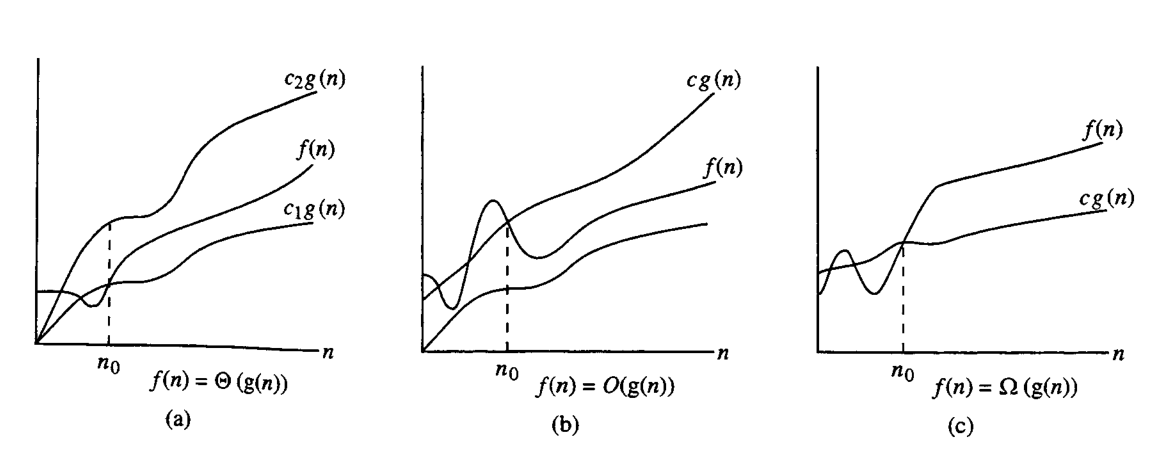
\includegraphics[width=11cm]{images/crescimento.png}
			
			{\bf Figura:} Comportamento das notações $\Theta$, $O$ e $\Omega$.
		\end{center}
	\end{frame}	
	
	\begin{frame}{Complexidade de Tempo}
		\begin{block}{$f_1 (n) = 5n^3 + 2n^2 + 22n + 6$}
			\begin{eqnarray}
			O(f_1(n)) & = & O(5n^3 + 2n^2 + 22n + 6)\\
			& = & O(5n^3)\\
			& = & O(n^3)
			\end{eqnarray}
		\end{block}   
		\begin{exampleblock}{É verdade porque...}
			Basta admitir $c = 6$, e $n_0 = 10$. Logo
			\begin{center}
				$5n^3 + 2n^2 + 22n + 6 \leq 6n^3$
			\end{center}
			para todo $n \geq 10$.
		\end{exampleblock}
	\end{frame}
	
	\begin{frame}{Complexidade de Tempo}
		\begin{block}{$f_1 (n) = 5n^3 + 2n^2 + 22n + 6$}
			\begin{eqnarray}
			O(f_1(n)) & = & O(5n^3 + 2n^2 + 22n + 6)\\
			& = & O(5n^3)\\
			& = & O(n^3)
			\end{eqnarray}
		\end{block}   
		\begin{exampleblock}{Também é verdade dizer que...}
			$f_1(n) = O(n^4)$, pois $n^4$ é maior que $n^3$ e portanto é ainda um limitante assintótico superior sobre $f_1$.
		\end{exampleblock}   
		\begin{alertblock}{Mas...}
			$f_1(n) \not= O(n^2)$.
		\end{alertblock}
	\end{frame}
	
	\begin{frame}{Complexidade de Tempo}
		\begin{block}{$f_2 (n) = \mbox{log}_{13} n + 5$}
			\begin{eqnarray}   
			O(f_2(n)) & = & O(\mbox{log}_{13} n + 5)\\
			& = & O(\mbox{log}_{13} n)\\
			& = & O(\mbox{log} n)
			\end{eqnarray}
		\end{block}   
		\begin{exampleblock}{Porque...}
			$\mbox{log} n = \mbox{log}_{10} n  = \frac{\mbox{log}_{13} n}{\mbox{log}_{13} 10}$
		\end{exampleblock}
	\end{frame}

	\section{Classe P}
	\begin{frame}{Complexidade de Tempo}
		\begin{block}{Definição 7.7}
			Seja $t: \mathbb{N} \rightarrow \mathbb{R}^+$ uma função. Defina a {\bf classe de complexidade de tempo}, {\bf TIME($t(n)$)}, como sendo a coleção de todas as linguagens que são decidíveis por uma máquina de Turing de tempo $O(t(n))$.
		\end{block} \pause
		\begin{block}{Exemplo}
			\begin{itemize}
				\item $A = \{ 0^k 1^k$ | $k \geq 0 \}$
				\item $A \in$ {\bf TIME($n^2$)}, pois \pause
				\item $M_1$ decide $A$ em tempo $O(n^2)$
			\end{itemize}
		\end{block}
	\end{frame}
	
	\begin{frame}[shrink]{Complexidade de Tempo}
		\begin{block}{Problema}
			Seja a linguagem $A = \{ 0^k 1^k$ | $k \geq 0 \}$. Quanto tempo uma máquina de Turing simples precisa para decidir $A$?
		\end{block} 
		\begin{block}{Descrição de uma possível MT simples}
			$M_1$ = ``Sobre a cadeia de entrada $\omega$:
			\begin{enumerate}
				\item Faça uma varredura na fita e {\it rejeite} se um 0 for encontrado à direita de um 1.
				\item Repita se ambos 0s e 1s permanecem sobre a fita:
				\begin{enumerate}
					\item Faça uma varredura na fita, cortando um único 0 e um único 1.
				\end{enumerate}
				\item Se 0s ainda permanecerem após todos os 1s tiverem sido cortados, ou se 1s ainda permanecerem após todos os 0s tiverem sido cortados, {\it rejeite}. Caso contrário, se nem 0s nem 1s permanecerem sobre a fita, {\it aceite}.
			\end{enumerate}
		\end{block}
	\end{frame}
	
	\begin{frame}{Complexidade de Tempo}
		\begin{block}{Problema}
			Existe uma máquina que decide assintoticamente \\a linguagem $A$ mais rapidamente?
		\end{block} \pause
		\begin{block}{Com outras palavras...}
			$A \in$ {\bf TIME($t(n)$)}, para algum $t(n) = o(n^2)$?
		\end{block}
	\end{frame}
	
	\begin{frame}[shrink]{Complexidade de Tempo}
		\begin{block}{Descrição de uma outra MT simples}
			$M_2$ = ``Sobre a cadeia de entrada $\omega$:
			\begin{enumerate}
				\item Faça uma varredura na fita e {\it rejeite} se um 0 for encontrado à direita de um 1.
				\item Repita enquanto alguns 0s e alguns 1s permanecem sobre a fita:
				\begin{enumerate}
					\item Faça uma varredura na fita, verificando se o número total de 0s e 1s remanescentes é par ou ímpar. Se for ímpar, {\it rejeite}.
					\item Faça uma varredura novamente na fita, \\cortando alternadamente um 0 não e outro sim \\(começando com o primeiro 0) \\e então cortando alternadamente um 1 não e outro sim \\(começando com o primeiro 1).
				\end{enumerate}
				\item Se nenhum 0 e nenhum 1 permanecer sobre a fita, {\it aceite}. Caso contrário, {\it rejeite}.
			\end{enumerate}
		\end{block}
	\end{frame}
	
	\begin{frame}{Complexidade de Tempo}
		\begin{block}{Problema}
			Podemos decidir a linguagem $A$ em tempo $O(n)$ \\(também chamado {\bf tempo linear})?
		\end{block} \pause
		\begin{exampleblock}{Sim... é possível!}
			Se utilizarmos uma máquina de Turing com duas fitas!
		\end{exampleblock}
	\end{frame}
	
	\begin{frame}[shrink]{Complexidade de Tempo}
		\begin{block}{Descrição de uma outra MT simples}
			$M_3$ = ``Sobre a cadeia de entrada $\omega$:
			\begin{enumerate}
				\item Faça uma varredura na fita e {\it rejeite} se um 0 for encontrado à direita de um 1.
				\item Faça uma varredura nos 0s sobre a fita 1 até o primeiro 1. \\Ao mesmo tempo, copie os 0s para a fita 2.
				\item Faça uma varredura nos 1s sobre a fita 1 até o final da entrada. Para cada 1 lido sobre a fita 1, corte um 0 sobre a fita 2. Se todos os 0s estiverem cortados antes que todos os 1s sejam lidos, {\it rejeite}.
				\item Se todos os 0s tiverem agora sido cortados, {\it aceite}. Se algum 0 permanecer, {\it rejeite}.
			\end{enumerate}
		\end{block}
	\end{frame}
	
	\subsection{Complexidade entre Modelos}	
	
	\begin{frame}{Relacionamentos de Complexidade entre Modelos}
		\begin{block}{Teorema 7.8}
			Seja $t(n)$ uma função, em que $t(n) \geq n$. Então toda máquina de Turing multifita de tempo $t(n)$ tem uma máquina de Turing de um única fita equivalente de tempo $O(t^2(n))$.
		\end{block} \pause
		\begin{block}{Teorema 7.11}
			Seja $t(n)$ uma função, em que $t(n) \geq n$. Então toda máquina de Turing não-determinística de uma única fita de tempo $t(n)$ tem uma máquina de Turing de um única fita equivalente de tempo $2^{O(t(n))}$.	
		\end{block}
	\end{frame}
	
	\begin{frame}{A Classe P}
		\begin{block}{Diferenças de complexidade de tempo}
			\begin{itemize}
				\item MT simples $x$ MT multi-fita: \\potência quadrática (ou {\it polinomial})
				\item MT simples $x$ MT não-determinística: \\no máximo {\it exponencial}.
			\end{itemize} 		
		\end{block}
	\end{frame}
	
	\begin{frame}{A Classe P}
		\begin{block}{Diferenças entre as taxas de crescimento}
			{\bf Exemplo:} $n^3$ e $2^n$ \pause
			\begin{itemize}
				\item Admita $n = 1000$; \pause
				\item Logo, $n^3 = 1$ bilhão; \pause
				\item Mas, $2^n$ é maior que o número de átomos do universo.
			\end{itemize}
		\end{block}
	\end{frame}
	
	\begin{frame}{A Classe P}
		\begin{block}{Definição 7.12}
			{\bf P} é a classe de linguagens que são decidíveis em tempo polinomial sobre uma máquina de Turing determinística de uma única fita. \\Em outras palavras
			\begin{center}
				{\bf P} = $\bigcup\limits_{k}$ {\bf TIME ($n^k$)}.
			\end{center}
		\end{block} \pause
		\begin{block}{{\bf P} é importante porque...} \pause
			\begin{itemize} 
				\item {\bf P} é invariante para todos os modelos de computação polinomialmente equivalentes à máquina de Turing determinística de uma única fita; \pause
				\item {\bf P} corresponde aproximadamente à classe de problemas que são realisticamente solúveis em um computador.
			\end{itemize}
		\end{block}
	\end{frame}
	
	\begin{frame}{A Classe P}
		\begin{block}{Problema do caminho em um grafo}
			$CAM = \{ \langle G, s, t \rangle \mbox{ | } G$ é um grafo direcionado que tem um caminho direcionado de $s$ para $t \}$.
		\end{block} \pause
		\begin{center}
			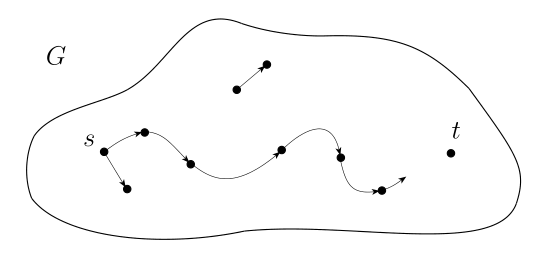
\includegraphics[width=8cm]{images/cam.png}
		\end{center}
	\end{frame}
	
	\begin{frame}{A Classe P}
		\begin{block}{Teorema 7.14}
			$CAM \in$ {\bf P}
		\end{block} \pause
		\begin{block}{Prova}
			$M$ = ``Sobre a cadeia de entrada $\langle G, s, t \rangle$ em que $G$ é um grafo direcionado com nós $s$ e $t$:
			\begin{enumerate}
				\item Ponha uma marca sobre o nó $s$.
				\item Repita o seguinte até que nenhum nó adicional seja marcado:
				\begin{enumerate}
					\item Faça uma varredura em todas as arestas de $G$. Se uma aresta $(a,b)$ for encontrada indo de um nó marcado $a$ para um nó não marcado $b$, marque o nó $b$.
				\end{enumerate}
				\item Se $t$ estiver marcado, {\it aceite}. Caso contrário, {\it rejeite}.
			\end{enumerate}
		\end{block}
	\end{frame}
	
	\begin{frame}
		\titlepage
	\end{frame}
	
\end{document}